\documentclass{article}

\usepackage[utf8]{inputenc}
\usepackage[T1]{fontenc}
\usepackage[hmargin=2.5cm,vmargin=3cm,bindingoffset=0.5cm]{geometry}

\usepackage{amsmath,amssymb}

\usepackage{graphicx}
\graphicspath{{figures/}}

\usepackage{float}
\usepackage{caption}
\usepackage{subcaption}

\usepackage{tikz}
\usetikzlibrary{arrows.meta, positioning, shapes.symbols}

\usepackage{xcolor,listings}
\definecolor{codegray}{RGB}{245,245,245}
\lstset{
  basicstyle=\ttfamily\small,
  backgroundcolor=\color{codegray},
  frame=single,
  numbers=left,
  numberstyle=\tiny,
  breaklines=true,
  captionpos=b,
  keywordstyle=\color{blue}\bfseries,
  commentstyle=\itshape\color{gray},
  stringstyle=\color{red!60!black},
  language=Python,
  literate=
    {→}{{$\rightarrow$}}2
    {≈}{{$\approx$}}2
    {≤}{{$\leq$}}2
    {≥}{{$\geq$}}2
    {–}{{--}}1
    {—}{{---}}1
}

\usepackage{booktabs}
\usepackage{longtable}
\usepackage{hyperref}
\hypersetup{
  colorlinks=true,
  linkcolor=blue!70!black,
  urlcolor=blue!70!black,
  citecolor=blue!70!black
}

\renewcommand{\lstlistingname}{Auflistung}

\begin{document}

\pagenumbering{alph}
\begin{titlepage}
  \begin{center}
    
\includegraphics[width=\textwidth]{THD-Logo.pdf}
    \vspace{1cm}
    \rule{\textwidth}{1mm}\\[0.3cm]
    \textsc{\scshape \huge Bachelor \,--\, Cyber Security}\\
    \rule{\textwidth}{1mm}\\[1.8cm]

    {\Large \bfseries Kryptologie 2}\\[1cm]
    {\Huge \bfseries Projektdokumentation}\\[0.5cm]
    {\Large \bfseries Cryptochallenge: CurveBall (CVE-2020-0601)}\\[2cm]

    \begin{minipage}[t]{0.45\textwidth}
      \begin{flushleft}
        \normalsize \emph{Autoren}\\
        Manuel Friedl – 12306626\\
        Christof Renner – 22301943
      \end{flushleft}
    \end{minipage}
    \hfill
    \begin{minipage}[t]{0.45\textwidth}
      \begin{flushright}
        \normalsize \emph{Betreuer}\\
        Prof.\,Dr.\,Martin Schramm
      \end{flushright}
    \end{minipage}\\[2cm]

    {\large Deggendorf, \today}
  \end{center}
\end{titlepage}

\newpage
\pagenumbering{Roman}
\tableofcontents
\newpage
\pagenumbering{arabic}

\section{Einleitung und Projektkontext}
\subsection{Motivation}
Die Schwachstelle \textbf{CurveBall} (CVE-2020-0601) in der Windows-CryptoAPI
ermöglicht es, X.509-Zertifikate mit manipulierten Elliptic-Curve-Parametern zu
signieren, sodass betroffene Windows-Versionen die Signaturen fälschlich als
gültig akzeptieren.\footnote{Microsoft Security Advisory ADV200002, 14.\,01.\,2020}
Im Modul \emph{Kryptologie 2} fehlte bislang ein modernes
Hands-On-Szenario, um diesen Fehler praktisch zu demonstrieren.

\subsection{Projektziele}
\begin{enumerate}
  \item \textbf{Didaktik}: Vollständiger Angriffszyklus von Discovery bis Exploit.
  \item \textbf{Sicherheit}: Deployment selbst muss trotz absichtlich verletzter Krypto sicher sein.
  \item \textbf{Portabilität}: Schnelle, plattformunabhängige Nutzung via Docker/Podman.
\end{enumerate}

\subsection{Bedrohungsmodell}
\begin{figure}[H]
  \centering
  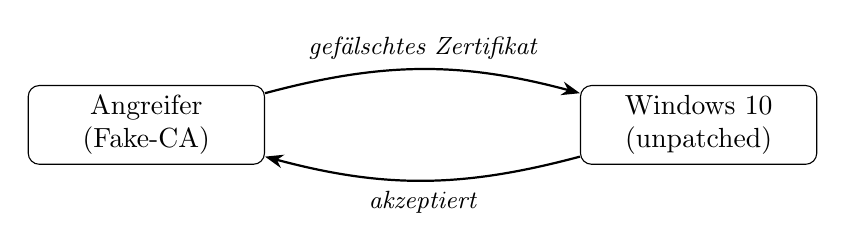
\begin{tikzpicture}[
      entity/.style={draw, rounded corners, align=center, minimum width=3cm, minimum height=1cm},
      arrow/.style={-Stealth, thick},
      label/.style={font=\small\itshape}
    ]
    \node[entity] (attacker) {Angreifer\\(Fake-CA)};
    \node[entity, right=4cm of attacker] (victim) {Windows 10\\(unpatched)};
    \path[arrow] (attacker) edge[bend left=15] node[label, above]{gefälschtes Zertifikat} (victim);
    \path[arrow] (victim) edge[bend left=15] node[label, below]{akzeptiert} (attacker);
  \end{tikzpicture}
  \caption{Simplifiziertes Threat-Model: fehlende Parameter-Validierung}
  \label{fig:threatmodel}
\end{figure}

\section{Herangehensweise}
\subsection{Zielsetzung}
\begin{itemize}
  \item Demonstration des Angriffs in einer kontrollierten Umgebung.
  \item Vermittlung von DevSecOps-Best-Practices (Linting, CI, Scans).
  \item Bereitstellung als \emph{„One-Click“}-Container, ohne lokale OpenSSL-Konfiguration.
\end{itemize}

\subsection{Methodik}
Wir arbeiteten in zwei Sprints à zwei Wochen.  
Abbildung~\ref{fig:process} zeigt den iterativen Ablauf.

\begin{figure}[H]
  \centering
  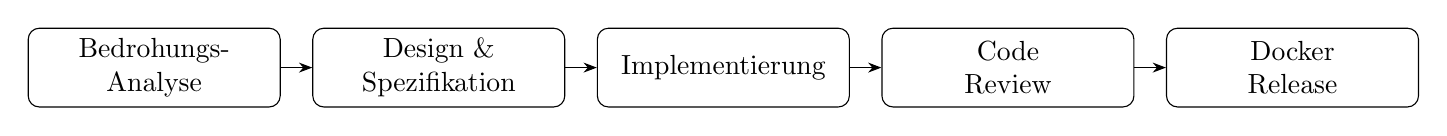
\begin{tikzpicture}[
      box/.style={draw, rounded corners, align=center, minimum width=3.2cm, minimum height=1cm},
      >=Stealth
    ]
    \node[box] (analyse) {Bedrohungs-\\Analyse};
    \node[box, right=0.4cm of analyse] (design) {Design \&\\Spezifikation};
    \node[box, right=0.4cm of design] (impl)  {Implementierung};
    \node[box, right=0.4cm of impl] (review) {Code\\Review};
    \node[box, right=0.4cm of review] (deploy) {Docker\\Release};

    \draw[->] (analyse) -- (design);
    \draw[->] (design) -- (impl);
    \draw[->] (impl) -- (review);
    \draw[->] (review) -- (deploy);
  \end{tikzpicture}
  \caption{Iterativer Projektablauf}\label{fig:process}
\end{figure}

\newpage

\subsection{Technisches Design}
Das technische Design der CurveBall-Challenge basiert auf einer modularen Web-Anwendung, die in Python mit Flask entwickelt wurde. Die Architektur folgt dem Model-View-Controller-Pattern und ist speziell darauf ausgelegt, kryptographische Konzepte interaktiv zu vermitteln.

\noindent
Die Anwendung besteht aus mehreren Kernkomponenten:

\begin{itemize}
  \item \textbf{Zertifikatsgenerator}: Python-Module zur Erstellung von X.509-Zertifikaten mit manipulierten ECC-Parametern
  \item \textbf{Validierungsengine}: Simulation der Windows CryptoAPI-Schwachstelle zur Demonstration fehlerhafter Zertifikatsprüfung
  \item \textbf{Web-Interface}: Interaktive Benutzeroberfläche für schrittweise Challenge-Durchführung
  \item \textbf{Visualisierungstools}: Grafische Darstellung von Zertifikatsinhalten und kryptographischen Parametern
\end{itemize}

\noindent
Die Challenge ist als Progressive Web Application konzipiert, die ohne Installation direkt im Browser läuft. Dabei wird besonderer Wert auf eine intuitive Benutzerführung gelegt, die auch Studierende ohne tiefgreifende Kryptographie-Kenntnisse abholt und schrittweise durch die komplexe Materie führt.

\subsection{Spielweise}
Die CurveBall-Challenge ist als interaktive Lernreise konzipiert, die Studierende spielerisch an das Thema heranführt.
\begin{enumerate}
  \item \textbf{Starten der Challenge}: Durch starten des Docker-Containers wird die Web-Anwendung bereitgestellt.
  \item \textbf{Aufrufen der Web-Anwendung}: Die Studierenden öffnen die Web-App im Browser unter \url{https://localhost:8443} und erhalten eine Einführung in die Challenge.
  \item \textbf{Einführung \& Theorie}: Vermittlung der Grundlagen zu elliptischen Kurven und X.509-Zertifikaten
  \item \textbf{Challenges}: Danach folgen verschiedene Herausforderungen, die die Studierenden dazu anregen, das Gelernte anzuwenden und zu vertiefen.
\end{enumerate}

\noindent
Jede Phase beinhaltet interaktive Elemente wie Code-Eingabefelder, Zertifikatsvisualisierungen und Validierungstools. Die Studierenden erhalten unmittelbares Feedback zu ihren Eingaben und können experimentell verschiedene Ansätze ausprobieren. Ein integriertes Hinweissystem bietet bei Bedarf gezielten Support, ohne die Lösung vorwegzunehmen.

\noindent
Die Challenge kann sowohl einzeln als auch in Kleingruppen bearbeitet werden und ist zeitlich flexibel gestaltbar – von kompakten 90-Minuten-Sessions bis zu mehrstündigen Vertiefungen.

\newpage
\section{Aufbau und Komponenten}
\subsection{Flask Webserver}
Der \emph{server.py} ist das Herzstück der Curveball CTF-Webanwendung und implementiert einen Flask-basierten Webserver mit SSL-Unterstützung. Der Server verwaltet 4 aufeinanderfolgende Challenges zum Thema ECC-Kryptographie und der CVE-2020-0601 Curveball-Schwachstelle.\\
\\
\textbf{Architektur und Technologie:}
\begin{itemize}
    \item \textbf{Framework:} Flask (Python Web Framework)
    \item \textbf{Session-Management:} Flask Sessions mit Secret Key
    \item \textbf{SSL/TLS:} HTTPS über Port 8443 mit eigenen Zertifikaten
    \item \textbf{Template Engine:} Jinja2 (Flask Standard)
\end{itemize}
\textbf{Kernfunktionalitäten:}
\begin{enumerate}
    \item \textbf{Challenge-Fortschrittsverfolgung}
    \begin{itemize}
        \item \textbf{Session-basiert:} Nutzt Flask Sessions zur Speicherung des Fortschritts
        \item \textbf{Sequenzieller Ablauf:} Challenges werden der Reihe nach freigeschaltet
        \item \textbf{Persistenz:} Fortschirtt bleibt während der Browser Session erhalten
    \end{itemize}
    \begin{lstlisting}[language=Python,caption={Challenge-Lock}]
    def is_challenge_unlocked(challenge_number):
    """Checks if a challenge is unlocked"""
        if challenge_number == 1:
            return True  # Challenge 1 is always unlocked
    
        completed = get_completed_challenges()
        # Challenge N is only available if Challenge N-1 is completed
        return (challenge_number - 1) in completed
    \end{lstlisting}
    \item \textbf{Route-Struktur}
    \begin{itemize}
        \item \textbf{Hauptrouten:}
        \begin{itemize}
            \item / => Startseite mit Challenge-Übersicht
            \item /introduction => Curveball-Einführung (Markdown zu HTML)
            \item /challenge1 bis /challenge4 => Einzelne Challenge-Seiten
        \end{itemize}
        \item \textbf{API-Endpunkte:}
        \begin{itemize}
            \item /api/complete\_challenge/<int> => Challenge als abgeschlossen markieren
            \item /api/challenge\_status => Aktueller Fortschrittsstatus
            \item /api/reset\_progress => Zurücksetzen des Fortschritts (Debug)
        \end{itemize}
        \item \textbf{Download-Endpunkte:}
        \begin{itemize}
            \item /downloads/<filename> => Challenge-Dateien (Zertifikate, JSON)
            \item /scripts/<filename> => Python-Skripte für Challenges
            \item /explain/<topic> => Kryptographie-Konzepte erklärt
        \end{itemize}
    \end{itemize}
    \item \textbf{Challenge-Inhalte}
    \begin{enumerate}
        \item \textbf{Challenge1:} ECC Grundlagen - Punktmultiplikation
        \item \textbf{Challenge2:} Zertifikatsanalyse mit OpenSSL
        \item \textbf{Challenge3:} Curveball Exploit Simulation
        \item \textbf{Challenge4:} Kurvenparameter \& Signaturvalidierung
    \end{enumerate}
\end{enumerate}

\subsection{Javascript}
Die CTF-Anwendung verwendet ein modulares JavaScript-System mit separaten Dateien für verschiedene Funktionsbereiche. Das System kombiniert mathematische ECC-Berechnungen, interaktive UI-Elemente und Fortschrittsverfolgung.\\

\subsubsection{main.js - Zentrale Steuerung}
\begin{itemize}
    \item \textbf{Funktion:} Grundlegende Seitenfunktionalität und Easter Egg
    \item \textbf{Features:}
    \begin{itemize}
        \item DOM-Initialisierung
        \item Konami-Code Implementation
        \item Visuelle Effekte (Gradient-Animation)
        \item Basis-Event-Handling
    \end{itemize}
\end{itemize}

\subsubsection{progress.js - Fortschrittssystem}
\begin{itemize}
    \item \textbf{Kernklasse:} ChallengeProgress
    \item \textbf{Funktionalitäten:}
    \begin{itemize}
        \item Session-basierte Fortschrittsverfolgung
        \item Server-API Integration
        \item Dynamische UI-Updates für Challenge-Cards
        \item Visuelle Status-Indikatoren (gesperrt/freigeschaltet/abgeschlossen)
    \end{itemize}
\end{itemize}

\subsubsection{challenge1.js - ECC Grundlagen}
\begin{itemize}
    \item \textbf{Thema:} Elliptische Kurven Punktmultiplikation
    \item \textbf{Kurvendefinition:} $y^2 = x^3 + 3$ (mod 97), Generator G = (11,3)
    \item \textbf{Mathematische Funktionen:}
    \begin{itemize}
        \item \emph{modInverse()} - Modulare Inverse Berechnung
        \item \emph{pointAdd()} - Elliptische Kurven Punktaddition
        \item \emph{scalarMult()} - Skalare Multiplikation
        \item \emph{isOnCurve()} - Punktvalidierung
    \end{itemize}
\end{itemize}

\subsubsection{challenge2.js - Zertifikatsanalyse}
\begin{itemize}
    \item \textbf{Thema:} Analysieren eines Zertifikats auf eine Flag
    \item \textbf{Max. Versuche:} 10 mit eskalierenden Hinweisen
    \item \textbf{Kernfunktionen:}
    \begin{itemize}
        \item Flag-Validierung mit mehreren Formatvarianten
        \item Progressives Hint-System nach mehreren Versuchen
        \item OpenSSL-Befehl-Kopierungsfunktion
        \item Confetti-Animationen bei Erfolg
        \item Lokale Speicherung des Fortschritts
    \end{itemize}
\end{itemize}

\subsubsection{challenge3.js - Curveball Exploit-Simulation}
\begin{itemize}
    \item \textbf{ECC-Kurven:} Unterstützung für P-256, P-384, P-521
    \item \textbf{Angriffsmethoden:}
    \begin{itemize}
        \item Generator-Punkt Manipulation
        \item Parameter-Spoofing
        \item Custom Exploits
        \item Confetti-Animationen bei Erfolg
        \item Lokale Speicherung des Fortschritts
    \end{itemize}
    \item \textbf{Kernfunktionen:}
    \begin{itemize}
        \item \emph{generateExploitParameters()} - Erstellt manipulierte Parameter
        \item \emph{generateRogueGenerator()} - Generiert manipulierte Generator-Punkte
        \item Mock-Zertifikatserstellung
        \item OpenSSL-Befehlsgenerierunng
    \end{itemize}
\end{itemize}

\subsubsection{challenge4.js - Kurvenparameter \& Signatur-Validierung}
\begin{itemize}
    \item \textbf{Standard-Kurve:} NIST P-256 Parameter
    \item \textbf{Max. Versuche:} 10 mit eskalierenden Hinweisen
    \item \textbf{Manipulationsmethoden:}
    \begin{itemize}
        \item Generator-Punkt Spoofing
        \item Kurvenparameter-Manipulation (a,b)
        \item Gruppenordnung-Manipulation (n)
        \item Benutzerdefinierte Kombinationen
    \end{itemize}
    \item \textbf{Kernfunktionen:}
    \begin{itemize}
        \item \emph{performManipulation()} - Führt Parameter-Manipulationen durch
        \item \emph{calculateExploitPotential()} - Bewertet Angriffspotenzial (0-100)
        \item Hex-Validierung und -Manipulation
        \item JSON-Export für Parameter
    \end{itemize}
\end{itemize}

\subsection{Python-Skript: verification.py}
Das Python-Skript verification.py dient als Simulator zur Analyse der Curveball-Schwachstelle (CVE-2020-0601) im Windows CryptoAPI. Es ermöglicht das Verständnis des fehlerhaften Verhaltens bei der ECC-Zertifikatsvalidierung, indem es zeigt, wie Windows in der betroffenen Version kritische Prüfungen – insbesondere die Validierung der ECC-Parameter und des Generatorpunkts – überspringt. Das Skript unterstützt zwei Betriebsmodi: einen Analysemodus, der die Unterschiede zwischen sicherer und unsicherer Validierung aufzeigt, sowie einen Validierungsmodus, mit dem manipulierte ECC-Zertifikate überprüft und potenzielle Exploit-Marker erkannt werden können. Durch die Simulation des Schwachstellenverhaltens bietet das Tool eine praxisnahe Möglichkeit zur Schulung und zum sicheren Testen von Sicherheitsmechanismen im Bereich der Zertifikatsprüfung. Bei erfolgreicher Ausnutzung wird eine symbolische Flagge ausgegeben, was das Skript auch für CTF-Challenges besonders geeignet macht.\\

\begin{lstlisting}[language=Python,caption={analyze\_ecc\_parameter()-Methode}]
    curve = public_key.curve
    curve_name = curve.name if hasattr(curve, 'name') else 'unknown'

    standard_curves = ['secp256r1', 'secp384r1', 'secp521r1']

    if curve_name not in standard_curves:
        return True, f"Non-standard curve detected: {curve_name}"

\end{lstlisting}
Im Rahmen der Schwachstellenanalyse überprüft das Skript, ob ein Zertifikat auf einer nicht standardisierten elliptischen Kurve basiert. Standardmäßig werden in der Praxis nur gut geprüfte Kurven wie \textbf{secp256r1}, \textbf{secp384r1} und \textbf{secp521r1} verwendet. Das Snippet extrahiert den Namen der verwendeten Kurve aus dem Zertifikat und vergleicht ihn mit dieser Liste. Wenn eine nicht standardisierte Kurve erkannt wird, deutet das auf eine manipulierte ECC-Struktur hin – ein zentrales Element der Curveball-Ausnutzung. Dadurch wird sichtbar, ob das Zertifikat potenziell Teil eines Exploits ist.\\

\subsection{Python-Skript: signature\_validator.py}
In diesem Skritp wird demonstriert, wie die Curveball-Schwachstelle (CVE-2020-0601) ausgenutzt werden kann, um gültige ECDSA-Signaturen auf Basis manipulierter elliptischer Kurvenparameter zu erzeugen – ohne Kenntnis des privaten Schlüssels. Im Zentrum steht die Klasse ECCSignatureValidator, die eine vereinfachte ECC-Signaturprüfung durchführt. Mithilfe manipulierten Parametersätzen lassen sich gezielt Situationen erzeugen, in denen Signaturen als gültig anerkannt werden, obwohl sie unter vertrauenswürdigen Parametern nicht gültig wären.\\
\\
Die Validierung beruht auf klassischen ECDSA-Schritten: Hashing der Nachricht, Inversion von s, Berechnung von Punktkombinationen auf der elliptischen Kurve und abschließender Vergleich.\\

\begin{lstlisting}[language=Python,caption={Punktmultiplikation auf der Kurve}]
def point_multiply(self, k: int, x: int, y: int) -> Tuple[int, int]:
    """Scalar multiplication on elliptic curve (simplified)"""
    if k == 0:
        return None, None
    if k == 1:
        return x, y

    result_x, result_y = None, None
    addend_x, addend_y = x, y

    while k:
        if k & 1:
            if result_x is None:
                result_x, result_y = addend_x, addend_y
            else:
                result_x, result_y = self.point_add(result_x, result_y, addend_x, addend_y)
        addend_x, addend_y = self.point_add(addend_x, addend_y, addend_x, addend_y)
        k >>= 1

    return result_x, result_y
\end{lstlisting}
Dieses Snippet implementiert das sogenannte Double-and-Add-Verfahren, um Punkte auf einer elliptischen Kurve effizient zu multiplizieren. Diese Operation ist zentral für die ECDSA-Signaturvalidierung und angreifbar, wenn die Kurvenparameter manipuliert werden.\\
\\
\begin{lstlisting}[language=Python,caption={Signaturprüfung mit Kurvenparametern}]
    final_x = result_x % self.order
    is_valid = final_x == signature_r
\end{lstlisting}
Der finale Schritt der Validierung vergleicht die x-Koordinate des berechneten Punkts mit dem übermittelten Signaturwert r. Wird durch manipulierte Parameter gezielt ein passender final\_x konstruiert, kann eine gefälschte Signatur als gültig erscheinen – Kern der Curveball-Ausnutzung.

\newpage
\section{Arbeitsaufteilung}

\noindent Die Arbeitsaufteilung erfolgte pragmatisch basierend auf den individuellen Stärken der Teammitglieder, wobei gleichzeitig Wert auf Wissenstransfer und gemeinsames Lernen gelegt wurde.

\begin{longtable}{|p{3cm}|p{5cm}|p{6cm}|}
    \hline
    \textbf{Teammitglied} & \textbf{Hauptaufgaben} & \textbf{Spezifische Aufgaben} \\
    \hline
    \endhead

    Manuel Friedl & Kryptographie \& Frontend & 
    \begin{itemize}
        \item Konzeptionierung der einzelnen Challenges
        \item Analyse der CVE-2020-0601 Schwachstelle
        \item Entwicklung der Python-Skripte \texttt{verification.py} und \texttt{signature\_validator.py} 
        \item Entwicklung des Web-Interface und Zertifikats-Visualizers
        \item Erstellung verständlicher Challenge-Beschreibungen
        \item Implementierung der Angriffslogik in Python
        \item Frontend-Design mit HTML/CSS
        \item Erstellen der Zertifikate \texttt{mystery\_cert.pem} und \texttt{valid\_certificate.pem}
        \item Dokumentation der kryptographischen Konzepte
    \end{itemize} \\
    \hline

    Christof Renner & DevOps \& Infrastruktur & 
    \begin{itemize}
        \item Konzeptionierung der einzelnen Challenges
        \item Docker-Containerisierung mit Multi-Stage-Builds
        \item CI/CD-Pipeline mit GitHub Actions
        \item Security-Scanning und Linting-Integration
        \item GitHub Container Registry Konfiguration
        \item Dokumentation der technischen Details
        \item Container-Deployment-Architektur
        \item Implementierung der Sicherheitsmaßnahmen
        \item Frontend-Optimierungen
    \end{itemize} \\
    \hline
    \end{longtable}

\noindent Dabei wurde durch regelmäßige Abstimmungen und gemeinsame Review-Sessions sichergestellt, dass alle Komponenten nahtlos zusammenarbeiten. Die technische Dokumentation wurde gleichmäßig zwischen beiden Teammitgliedern aufgeteilt, wobei jeder etwa 50\% der Dokumentationsarbeit übernahm.

\newpage

\section{Containerisierung}
\subsection{Dockerfile}
Das vorliegende Dockerfile definiert die Containerisierung der Curveball-CTF Webanwendung und nutzt dabei Python 3.12 auf Alpine Linux als schlanke und sicherheitsorientierte Basis. Durch die explizite Installation von OpenSSL Version 3.5.1-r0 werden kryptographische Funktionalitäten bereitgestellt, die für die SSL/TLS-basierten Challenges essentiell sind. Die Anwendung wird systematisch aufgebaut, indem zunächst die Python-Abhängigkeiten aus der \emph{requirements.txt} installiert werden, bevor der Anwendungscode kopiert wird - eine bewährte Praxis für effizientes Docker Layer Caching. Der Container exponiert Port 8443, einen Standard-Port für HTTPS-Verbindungen, und startet automatisch den Python-Server über das \emph{server.py}-Skript. Diese Konfiguration gewährleistet eine reproduzierbare, isolierte Umgebung für die Kryptologie-Challenges und minimiert gleichzeitig durch die Alpine-Basis die Angriffsfläche des Systems.

\vspace{1cm}

\begin{lstlisting}[language=bash,caption={Auszug aus dem finalen Dockerfile}]
FROM python:3.12-alpine

# Pin Alpine package versions for reproducible builds
RUN apk add --no-cache openssl=3.5.1-r0

WORKDIR /app
COPY requirements.txt /app/
RUN pip install --no-cache-dir --requirement requirements.txt

COPY . /app

EXPOSE 8443

CMD ["python", "server.py"]

\end{lstlisting}

\subsection{Architektur}
\begin{figure}[H]
  \centering
  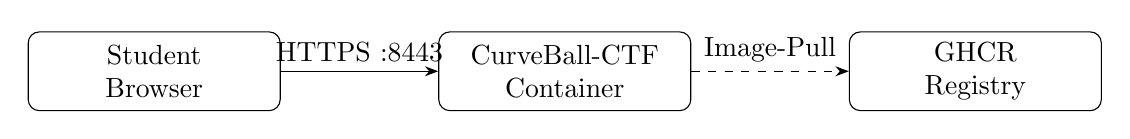
\begin{tikzpicture}[
      service/.style={draw, rounded corners, minimum width=3.2cm, minimum height=1cm, align=center},
      node distance=2cm
    ]
    \node[service] (browser) {Student\\Browser};
    \node[service, right=of browser] (ctf) {CurveBall-CTF\\Container};
    \node[service, right=of ctf] (registry) {GHCR\\Registry};

    \draw[-Stealth] (browser) -- node[midway, above]{HTTPS :8443} (ctf);
    \draw[-Stealth, dashed] (ctf) -- node[midway, above]{Image-Pull} (registry);
  \end{tikzpicture}
  \caption{Container-Deployment in der Lehrumgebung}\label{fig:container}
\end{figure}

\newpage

\section{CI/CD-Pipeline}

\subsection{Docker Build-Pipeline}
\noindent
Die automatisierte Erstellung und Veröffentlichung der Docker-Images erfolgt über eine dedizierte GitHub Actions Workflow-Datei. Diese Pipeline stellt sicher, dass bei jeder Aktualisierung des Codes oder auf manuelle Anforderung ein neues, konsistentes Container-Image erstellt und in die Docker Hub Registry hochgeladen wird.
\noindent
Der Workflow ist so konfiguriert, dass er manuell über die GitHub-Oberfläche ausgelöst werden kann (\texttt{workflow\_dispatch}), was besonders während der Entwicklungsphase und für kontrollierte Releases nützlich war.

\begin{lstlisting}[language=python,caption={Docker Build \& Publish Workflow}]
name: Build and Publish Docker image

on:  
  workflow_dispatch:

jobs:
  build-and-push:
    runs-on: ubuntu-latest

    steps:
      - name: Checkout repository
        uses: actions/checkout@v4

      - name: Set up Docker Buildx
        uses: docker/setup-buildx-action@v3

      - name: Log in to Docker Hub
        uses: docker/login-action@v3
        with:
          username: ${{ secrets.DOCKERHUB_USERNAME }}
          password: ${{ secrets.DOCKERHUB_TOKEN }}

      - name: Build and push Docker image
        uses: docker/build-push-action@v6
        with:
          context: ./curveball-ctf/webserver
          file: ./curveball-ctf/webserver/Dockerfile
          push: true
          tags: crnnr/curveball-cve-2020-0601:latest
\end{lstlisting}

\noindent
\textbf{Die Pipeline besteht aus mehreren wichtigen Schritten:} \\
\\
\noindent
Durch diese Automatisierung wird der Release-Prozess erheblich vereinfacht und gleichzeitig sichergestellt, dass jedes veröffentlichte Image den gleichen, reproduzierbaren Build-Prozess durchlaufen hat. \\
\\
Die Verwendung von gesicherten Secrets für die Authentifizierung erhöht zusätzlich die Sicherheit der Pipeline.
\noindent
Die Container-Registry fungiert als zentrales Repository für die fertigen Images, was die Verteilung an Studierende erheblich vereinfacht. \\ 
\\
Mit einem einfachen \texttt{docker pull} Befehl können Dozenten und Studenten die aktuelle Version der Challenge beziehen.

\newpage

\subsection{Linting‐Tools}

Für die Code-Qualität und Sicherheit setzen wir auf etablierte Tools:

\begin{itemize}
  \item \textbf{pylint}: Python-Code-Analyse nach PEP8
  \item \textbf{hadolint}: Dockerfile-Best-Practices
\end{itemize}

Diese Tools sind in der CI-Pipeline integriert und prüfen den Code bei jedem Commit. 

\begin{lstlisting}[language=python,caption={pylint.yml}]
jobs:
  build:
    runs-on: ubuntu-latest
    strategy:
      matrix:
        python-version: ["3.8", "3.9", "3.10"]
    steps:
    - uses: actions/checkout@v4
    - name: Set up Python ${{ matrix.python-version }}
      uses: actions/setup-python@v5
      with:
        python-version: ${{ matrix.python-version }}
    - name: Install dependencies
      run: |
        python -m pip install --upgrade pip
        pip install pylint
    - name: Analysing the code with pylint
      run: |
        pylint $(git ls-files '*.py')
\end{lstlisting}

\noindent
Damit konnte am Ende ein \textbf{pylint}-Score von \textbf{9.5/10} erreicht werden, was dafür sorgt, dass der Code auch in Zukunft gut lesbar und wartbar bleibt.

\subsection{Dockerfile-Linting}
\noindent
Die Dockerfile-Qualität wird mit \textbf{hadolint} geprüft, um Best Practices zu gewährleisten.
Das Linting erfolgt ebenfalls in der CI-Pipeline, um sicherzustellen, dass das Dockerfile den Standards entspricht.

\begin{lstlisting}[language=python,caption={hadolint.yml}]
jobs:
  hadolint:
    name: Hadolint
    runs-on: ubuntu-latest

    steps:
      - name: Checkout code
        uses: actions/checkout@v4

      - name: Set up Docker Buildx
        uses: docker/setup-buildx-action@v2

      - name: Run Hadolint
        uses: hadolint/hadolint-action@v2
        with:
          dockerfile: ./Dockerfile
\end{lstlisting}

\newpage

\subsection{Sicherheits-Scans}
Die Sicherheitsüberprüfung erfolgt mit \textbf{Bandit} und \textbf{Snyk}.
Bandit analysiert Python-Code auf Sicherheitslücken, während Snyk Container-Images auf bekannte Schwachstellen prüft.
Bandit ist in der CI-Pipeline integriert und prüft den Code bei jedem Commit.

\begin{lstlisting}[language=python,caption={bandit workflow file}]
jobs:
  bandit:
    name: Bandit Scan
    runs-on: ubuntu-latest

    steps:
      - name: Checkout code
        uses: actions/checkout@v4

      - name: Set up Python
        uses: actions/setup-python@v4
        with:
          python-version: '3.x'
      - name: Install Bandit
        run: |
          python -m pip install --upgrade pip
          pip install bandit

      - name: Run Bandit security scan
        run: |
          # scan the repo recursively instead of using stdin
          bandit -r . --skip trojansource
\end{lstlisting}

\noindent
Damit wird sichergestellt, dass der Code und die Container-Images regelmäßig auf Sicherheitslücken
überprüft werden. Die Ergebnisse der Scans werden in der CI-Pipeline angezeigt.
\noindent
Hierbei wurden einige Schwachstellen identifiziert:

\begin{lstlisting}[language=python,caption={bandit scan results}]
Code scanned:
	Total lines of code: 602
	Total lines skipped (#nosec): 0
	Total potential issues skipped due to specifically being disabled (e.g., #nosec BXXX): 0

Run metrics:
	Total issues (by severity):
		Undefined: 0
		Low: 6
		Medium: 1
		High: 1
	Total issues (by confidence):
		Undefined: 0
		Low: 0
		Medium: 3
		High: 5
\end{lstlisting}

\newpage

\noindent
Die identifizierten Schwachstellen sind folgendermassen verteilt:

\begin{figure}[H]
  \centering
  \begin{tabular}{|l|l|l|l|}
    \hline
    \textbf{Severity} & \textbf{Confidence} & \textbf{Issue Type} & \textbf{Anzahl} \\
    \hline
    High & High & B105: hardcoded\_password\_string & 1 \\
    \hline
    Medium & High & B101: assert\_used & 1 \\
    \hline
    Low & High & B311: random & 3 \\
    \hline
    Low & Medium & B404: import\_subprocess & 1 \\
    \hline
    Low & Medium & B603: subprocess\_without\_shell\_equals\_true & 1 \\
    \hline
    Low & Medium & B607: start\_process\_with\_partial\_path & 1 \\
    \hline
  \end{tabular}
  \caption{Bandit Security Scan Ergebnisse -- Identifizierte Schwachstellen nach Severity und Confidence}
  \label{fig:bandit}
\end{figure}

Diese Schwachstellen wurden im Rahmen der Entwicklung analysiert und entsprechend dem Projektkontext bewertet:

\begin{itemize}
  \item \textbf{B404: import\_subprocess}: Die referenziert die Verwendung von \texttt{subprocess} in sicherheitskritischen Bereichen. Hier wurde sichergestellt, dass alle Eingaben validiert werden, um potenzielle Angriffe zu verhindern.

  \item \textbf{B607: start\_process\_with\_partial\_path}: Diese Warnung bezieht sich auf die Verwendung von relativen Pfaden beim Starten von Prozessen. Um das Risiko von Pfadmanipulationen zu minimieren, wurde darauf geachtet, dass alle Pfade nicht relativ sind und keine Benutzereingaben direkt in Pfade einfließen.

  \item \textbf{B603: subprocess\_without\_shell\_equals\_true}: Diese Warnung bezieht sich auf die Verwendung von \texttt{subprocess} ohne die Option \texttt{shell=True}. Hier wurde sichergestellt, dass alle Aufrufe von \texttt{subprocess} sicher sind und keine Shell-Injection-Angriffe möglich sind.

  \item \textbf{B201: flask\_debug\_true}: Diese Warnung bezieht sich auf die Verwendung von \texttt{flask} im Debug-Modus. In einer produktiven Umgebung sollte der Debug-Modus deaktiviert werden, um potenzielle Sicherheitsrisiken zu minimieren.

  \item \textbf{B104: hardcoded\_bind\_all\_interfaces}: Bezieht sich auf die Konfiguration des Flask-Servers, der auf allen Schnittstellen lauscht. Dies ist für die Challenge-Umgebung akzeptabel, da sie in einer kontrollierten Umgebung läuft und nicht öffentlich zugänglich ist.
\end{itemize}

\noindent
Doppelte Warnungen wurden im Rahmen der Entwicklung analysiert und entsprechend dem Projektkontext bewertet.
\noindent
Die bewusste Entscheidung, bestimmte Bandit-Warnungen im Challenge-Kontext zu akzeptieren, wurde dokumentiert und entspricht dem Projektcharakter als kontrollierte Lernumgebung.
\newpage

\section{Nicht umgesetzte VM-Erweiterung}
Ursprünglich war eine vorgefertigte Windows 10-VM (Version 1909, ungepatcht) als zentraler Bestandteil des Projekts geplant,
um den CurveBall-Angriff vollständig bis zum System-Rootstore zu demonstrieren und eine authentische Angriffsumgebung zu schaffen.
Diese VM hätte es ermöglicht, die realen Auswirkungen eines erfolgreichen Angriffs unmittelbar zu beobachten, einschließlich der
Manipulation von HTTPS-Verbindungen und Code-Signatur-Verifikationen.

\subsection{Herausforderungen bei der VM-Implementierung}
Die Umsetzung dieses Ansatzes scheiterte letztendlich aus mehreren gravierenden Gründen:

\begin{description}
  \item[Licensing-Problematik] Die Weitergabe eines vorinstallierten Windows-Images verstößt eindeutig gegen die Microsoft End User License Agreement (EULA). Eine rechtskonforme Lösung hätte erfordert, dass jeder Teilnehmer eine eigene Windows-Lizenz einbringt und selbst eine Installation durchführt, was den niederschwelligen Zugang zur Übung erheblich erschwert hätte.
  
  \item[Storage-Anforderungen] Das vollständige Windows 10-Image hätte mindestens 8 GB Speicherplatz benötigt, selbst in komprimierter Form. Dies hätte den Rahmen des Git-Repositorys gesprengt und eine Nutzung von Git LFS (Large File Storage) erforderlich gemacht, was mit erheblichen Kosten für Bandbreite und Speicherplatz verbunden gewesen wäre. Zudem hätte die Verteilung an mehrere Dutzend Studierende die Netzwerkressourcen der Hochschule stark belastet.
  
  \item[CI/CD-Limitationen] Die genutzten GitHub-Actions-Runner unterstützen keine Nested-Virtualisation, was eine automatisierte Überprüfung und Tests der VM innerhalb der CI/CD-Pipeline unmöglich machte. Dies hätte zu nicht getesteten Releases führen können, was dem DevSecOps-Ansatz des Projekts fundamental widerspricht.
\end{description}

\subsection{Vorteile der Container-Lösung}
Die stattdessen implementierte Container-Variante bietet mit rund 280 MB eine um mehr als 96\% reduzierte Größe im Vergleich zur VM-Lösung. 
Diese drastische Reduktion ermöglicht:

\begin{itemize}
  \item \textbf{Schnellere Deployments}: Studierende können das Image in Sekunden statt Minuten herunterladen
  \item \textbf{Plattformunabhängigkeit}: Funktioniert auf Windows, macOS und Linux ohne Anpassungen
  \item \textbf{Geringere Systemanforderungen}: Läuft auf nahezu jedem Rechner, der Docker unterstützt
  \item \textbf{Einfache Integration in CI/CD}: Vollständige Testabdeckung in der Entwicklungspipeline
  \item \textbf{Reproduzierbare Builds}: Jeder Build erzeugt identische Umgebungen
\end{itemize}

\newpage

\section{Ausblick}
Die entwickelte Container-Lösung bildet eine solide Grundlage für weitere Erweiterungen des Projekts. Folgende Weiterentwicklungen sind für zukünftige Versionen angedacht:

\begin{enumerate}
  \item \textbf{Windows-Live-Lab über Azure Lab Services}: 
  \begin{itemize}
    \item Bereitstellung von echten, identisch konfigurierten Windows-Hosts in verschiedenen Patch-Zuständen (vor und nach CVE-2020-0601-Patch)
    \item Integration einer kontrollierten Internet-Umgebung zum Testen realer TLS-Verbindungen
    \item Automatisierte Provisioning-Lösung mit Infrastructure-as-Code (Terraform/ARM-Templates)
    \item Zeitgesteuerte Verfügbarkeit zur Kostenoptimierung und Ressourcenschonung
    \item Zentrale Überwachungsmöglichkeiten für Dozenten zur Bewertung des Lernfortschritts
  \end{itemize}
  
  \item \textbf{Automatisierte Angriffskette}: 
  \begin{itemize}
    \item Integration von Browser-Automation mit Playwright/Selenium für einen vollständigen End-to-End-Exploit
    \item Demonstration der Auswirkungen auf verschiedene Browserfamilien (Chromium, Firefox, Safari)
    \item Simulation eines Man-in-the-Middle-Angriffsszenarios mit TLS-Interception
    \item Visualisierung der Angriffsphasen mit interaktivem Ablaufdiagramm
    \item Erweiterung um zusätzliche Krypto-Angriffe (etwa ALPACA oder BEAST) für umfassendere Lernszenarien
  \end{itemize}

\end{enumerate}

\newpage

\section{Fazit}
Unser Projekt demonstriert eindrucksvoll, wie sich ein kritischer kryptographischer Schwachpunkt wie CurveBall (CVE-2020-0601) in eine didaktisch wertvolle, aber dennoch sichere Lernumgebung überführen lässt. Die entwickelte Lösung schlägt erfolgreich die Brücke zwischen theoretischem Verständnis und praktischer Anwendung im Bereich der Kryptographie.

\subsection{Erreichte Ziele}
Die Containerisierung des Projekts ermöglicht einen niederschwelligen Zugang zur komplexen Thematik der Elliptischen-Kurven-Kryptographie und deren potentieller Schwachstellen. Dabei wurden alle initial definierten Projektziele erreicht:

\begin{itemize}
  \item \textbf{Didaktischer Mehrwert}: Die Studierenden können den vollständigen Angriffszyklus von der theoretischen Grundlage bis zur praktischen Exploitation nachvollziehen und selbst durchführen.
  
  \item \textbf{Sicherheitskonzept}: Trotz der absichtlich integrierten kryptographischen Schwachstelle ist das Deployment selbst durch die Containerisierung und strikte Isolation inhärent sicher gestaltet.
  
  \item \textbf{Plattformunabhängigkeit}: Die Docker/Podman-basierte Lösung garantiert eine konsistente Erfahrung über verschiedene Betriebssysteme und Hardwarekonfigurationen hinweg.
\end{itemize}

\subsection{Kompetenzerwerb}
Neben dem technischen Verständnis für die CurveBall-Schwachstelle erwerben die Studierenden durch die Auseinandersetzung mit dem Projekt wesentliche Kompetenzen in:

\begin{itemize}
  \item Grundlagen der Public-Key-Infrastruktur und X.509-Zertifikaten
  \item Praktischer Anwendung von kryptographischen Bibliotheken (OpenSSL, cryptography)
  \item Nutzung und Verständnis moderner DevSecOps-Workflows und CI/CD-Pipelines
  \item Containerisierung und Deployment von Anwendungen
  \item Sicherheitsrelevanten Best Practices in der Softwareentwicklung
\end{itemize}

\subsection{Langfristiger Nutzen}
Die entwickelte Lösung stellt nicht nur ein temporäres Lernmittel dar, sondern kann als wiederverwendbare Plattform für zukünftige kryptographische Szenarien dienen. Der modular aufgebaute Container und die umfassende Dokumentation ermöglichen eine einfache Erweiterung und Anpassung an neue Anforderungen oder andere kryptographische Schwachstellen.

Die Integration von DevSecOps-Praktiken in das Projekt selbst vermittelt den Studierenden zusätzlich einen Einblick in die heute in der Industrie etablierten Sicherheitsstandards und Workflows, was einen wertvollen Praxisbezug herstellt und die Employability der Absolventen steigert.

\end{document}
